\section{Robotics Framework for Reliable Trajectory Execution}\label{sec:architecture}

\subsection{Notations}

Before describing the robot architecture, let us introduce the
following notations:

\begin{description}
\item[$\text{SE}(2)$ and $\text{SE}(3)$]\hspace{1.45cm} the Special
  Euclidian groups of dimension 2 and 3 denotes rigid transformations
  in the 2d and 3d Euclidian spaces.
\item[$\mathbf{\bar{q}}(t)$] denotes the robot configuration in its
  configuration space $\mathcal{\bar{C}}$ at time $t$. It is divided
  into a controllable part $\mathbf{q}(t) \in \mathcal{C}$ and the
  robot position $\mathbf{x}(t) \in \text{SE}(3)$. The robot position
  is defined as the position of a particular robot body. In this
  paper, we chose the left ankle as the reference body used to compute
  the robot position. $\mathbf{\dot{q}(t)}$ describes the joint
  velocities.
\item[$\mathbf{x}_{\text{ref}}(t) \in \text{SE}(3)$] \hspace{1.2cm} is
  the robot planned trajectory.
\item[$\mathbf{\hat{x}}(t) \in \text{SE}(3)$] \hspace{.8cm} is the
  robot trajectory as perceived by the localization system.
\item[$\mathbf{c}(t) \in \mathbb{R}^2$ and $\mathbf{z}(t) \in
  \mathbb{R}^3$]\hspace{2.6cm} are respectively the projection of the
  robot center of mass on the floor ($z = 0$) and the Zero Momentum
  Point position at time $t$.
\item[$\mathbf{\gamma_{\text{la}}}(t) \in \text{SE}(3)$, $\mathbf{\gamma_{\text{ra}}}(t)
  \in \text{SE}(3)$]\hspace{3.4cm} denote respectively left ankle and
  right ankle trajectories.
\item[$\theta(t) \in \text{SE}(3)$]\hspace{0.8cm} is the estimated
  camera pose at time $t$.
\end{description}

The set of trajectories $\mathbf{\gamma_{\text{la}}}$,
$\mathbf{\gamma_{\text{ra}}}$ and $\mathbf{c}$ define a complete
balanced walking movement and is denoted $\mathbf{\Gamma}$. It can be
completed by an additional trajectory which define the upper-body
configuration during the walk. Changes in the upper-body posture do
not impact the walking movement as long as the center of mass
trajectory is respected. Therefore, this article will not mention
upper-body trajectory although the final experiment contains arms and
head movement.

\subsection{Robotics Architecture}

The proposed architecture can be divided in two parts:
\begin{enumerate}
\item The vision processing and localization components which are
  responsible for acquiring data on the two robots camera, computing
  an estimation of the camera pose and deducing the robot
  localization.
\item The control system which follows the planned trajectory while
  closing the loop on the localization data.
\end{enumerate}

These two systems are running on two different computers embedded on
the robot. They are composed of several robotics components running
simultaneously. Fig.~\ref{fig:framework_overview} illustrates the
complete robotics infrastructure. To communicate, we rely heavily on
both OpenHRP and ROS middlewares.
%
\begin{figure}[ht!]
  \begin{center}
    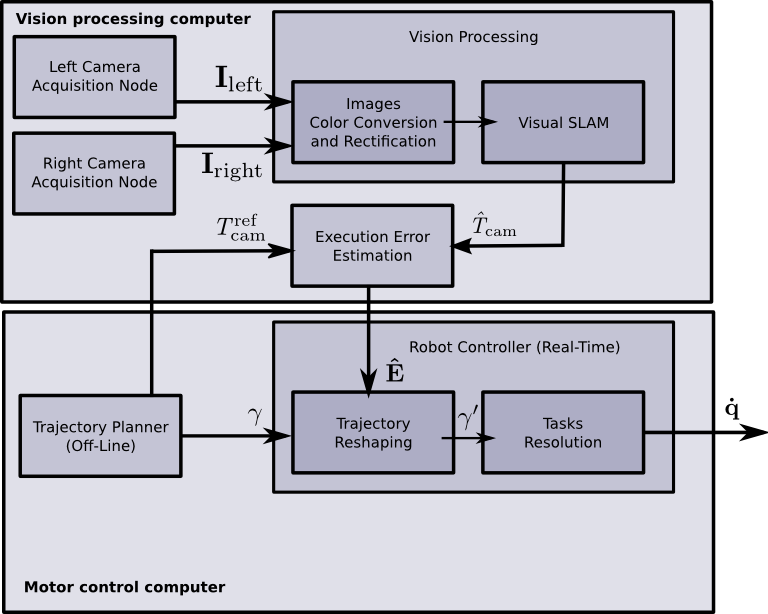
\includegraphics[width=\linewidth]{images/rss_framework.png}
  \end{center}
  \caption{Complete robotics framework overview. Let
    $\mathbf{I}_{\text{left}}$, $\mathbf{I}_{\text{right}}$ be
    respectively the left and right camera
    images. $\mathit{T}_{\text{cam}}$, $\mathit{\hat{T}}_{\text{cam}}$
    respectively the planned and estimated camera
    position. $\mathbf{\gamma}$ the concatenation of the left ankle,
    right ankle, upper body and center of mass
    trajectories. $\mathbf{\gamma'}$ the trajectories reshaped by
    taking into account execution
    errors.\label{fig:framework_overview}}
\end{figure}

\paragraph{Vision-based localization}

The vision system relies on two Flea2 FireWire cameras. They have been
set up to grab monochrome images synchronously at 30\hertz. The image
resolution is $320 \times 240$.

Images are transmitted to the vision component. It is in charge of
image rectification and current camera pose computation. This process
is described in detail in section~\ref{sec:vision}.  During our
experiments, the pose estimation rate was around 16\hertz.


\paragraph{Error estimation}

The error estimation component computes $\mathbf{\delta x} \in
\text{SE}(3)$, the transformation from the perceived robot position to
the planned robot position and is defined at time $t$ as:

\begin{equation} \label{eq:errorpos}
  \mathbf{\delta x}_t = \mathbf{x}_t . \hat{\mathbf{x}}_t^{-1}
\end{equation}

However, $\hat{\mathbf{x}}_t^{-1}$ is not directly provided by the
localization which estimates the camera pose and not the robot
pose. The transformation from the camera to the left ankle (defining
the robot position) can be easily deduced from the control and is not
subject to significant execution errors as joint encoders allow
low-level reliable servoing.

Additionally, the control is used to help the camera pose
estimation. Indeed, to estimate a 3d pose, it is necessary to estimate
six parameters; three for the translation: $x$, $y$, $z$ and three for
the rotation: roll, pitch, and yaw. Nevertheless, we know for sure
that the camera height $z$ and two of the three parameters of the
rotation cannot drift nor have significant execution errors while
walking on a flat ground. This explains why, in practice, only three
parameters are estimated using the vision components whereas the $z$,
roll and pitch parameters are known from the plan.

\paragraph{Closed-loop trajectory following}

To achieve walking and compute motor control, the task based control
framework described in~\cite{Mansard09icar} is used. One interesting
feature of this approach is that we can directly add tasks to follow
ankles and center of mass reference trajectories. The inverse
kinematics computation will then be implicitly realized by the task
resolution.

Regarding trajectory generation, we use the planner described in
\cite{Dalibard11humanoids} to generate the required reference
trajectories.

Our control scheme adds an additional step which processes the
reference trajectories to compensate for execution errors based on the
error estimation.

Let us consider that at time $t$, the robot is on double support
(i.e.\ both feet on the ground) and that an estimation of the
execution error $\mathbf{\delta \mathbf{x}}(t)$ is available. We have
to alter the trajectories of the left ankle, right ankle and center of
mass simultaneously while preserving robot balance. As we cannot
change a foot position while it is on contact with the floor, we have
to modify the trajectories during the two following steps to be able
to correct both feet trajectories. To do so, we will sum each
trajectory with a trajectory dependent third order polynomial denoted
by $\mathbf{\Delta}_{\text{la}} \in \text{SE(3)}$,
$\mathbf{\Delta}_{\text{ra}} \in \text{SE(3)}$,
$\mathbf{\Delta}_{\mathbf{c}} \in \mathbb{R}^2$:

\begin{equation}
  \begin{aligned}
    \mathbf{\gamma}'_{\text{la}}(t) = \mathbf{\Delta}_{la}(t) . \mathbf{\gamma}'_{\text{la}}(t)\\
    \mathbf{\gamma}'_{\text{ra}}(t) = \mathbf{\Delta}_{ra}(t) . \mathbf{\gamma}'_{\text{ra}}(t)\\
    \mathbf{c}'(t) = \mathbf{\Delta}_{c}(t) + \mathbf{c}(t)
  \end{aligned}
  \label{eq:cst_delta}
\end{equation}

Let $t_1$ be the end of the next step and $t_2$ the end of the second
next step. If the first step is realized with the left foot (i.e.\ the
right foot is the support foot). In Eq.~\ref{eq:cst_delta}, if
$\Delta$ provides a correction from $t_{\text{start}}$ to
$t_{\text{end}}$, we consider the following constraints:

\begin{equation}
\begin{aligned}
  \mathbf{\Delta}(t) =
  \begin{cases}
    0.,  & \mbox{if }t\mbox{$\leq t_{\text{start}}$} \\
    \mathbf{\delta x}, & \mbox{if }t\mbox{$\geq t_{\text{end}}$}
  \end{cases}\\
  \frac{\partial \mathbf{\Delta}}{\partial t}(t_1) = \frac{\partial
    \mathbf{\Delta}}{\partial t}(t_2) &= 0
\end{aligned}
\label{eq:deltaConstraints}
\end{equation}

The constraints expressed in Eq.~\ref{eq:deltaConstraints} insures
that the correction is smooth: null velocity at the beginning and end
of the correction and that the error is correctly compensated. They
are independent from the corrected trajectory (ankles or center of
mass). These four constraints fully determine the four coefficients of
the polynomial.

The starting and timing correction time depends on the corrected trajectory:
\begin{description}
\item[center of mass ($\mathbf{\Delta_c}(t)$):]\hspace{3cm}
  $t_{\text{start}} = t$,~~$t_{\text{end}} = t_1$
\item[left ankle ($\mathbf{\Delta_{\text{la}}}(t)$):]\hspace{3cm}
  $t_{\text{start}} = t$,~~$t_{\text{end}} = t_1$
\item[right ankle ($\mathbf{\Delta_{\text{ra}}}(t)$):]\hspace{3cm}
  $t_{\text{start}} = t_1$, $t_{\text{end}} = t_2$
\end{description}


The remaining issue is insuring that the updated trajectory will be
balanced. A classical approach is using the Zero Momentum Point: this
virtual point acts as a criterion to determine whether a trajectory is
balanced or not. If it lies in the convex hull of the robot contact
points all the time, the trajectory is balanced, otherwise it is
not. The ZMP is defined as:
%
\begin{equation} \label{eq:zmp1}
  \mathbf{z} = \mathbf{c} + \frac{1}{m(\ddot{c}_z +
    g)}\left(\begin{array}{ccc} 0 &-1 &0\\1 &0 &0\end{array}\right)
    \mathbf{\dot{\textbf{L}}} - \frac{c_z}{\ddot{c}_z + g}
    \ddot{\mathbf{c}}
\end{equation}
%
where $c_z$ is the height of the center of mass with respect to the
ground, $m$ is the mass of the robot, $g$ is the gravity constant,
\mbox{$\mathbf{c}=(c_x,c_y)$} is the projection of the center mass of
the robot on the ground and $\textbf{L}$ is the angular momentum of
the robot about the center of mass.


Solving this equation is time consuming as it is non-linear and
requires dynamics computation. Under additional assumptions detailed
in~\cite{Kajita01iros}, we can obtain a simplified linear model:
%
\begin{equation} \label{eq:zmp2}
  \mathbf{z} = \mathbf{c} - \frac{\mathbf{c}_z}{g} . \ddot{\mathbf{x}}
\end{equation}
%
Considering $\mathbf{r}$ a polynomial depending only of $\mathbf{z}$,
$(V_x, V_y, W_x, W_y)$ free parameters used to constrain the initial
position and velocity of the center of mass, a general solution of
Eq.~\ref{eq:zmp2} is:
%
\begin{equation} \label{eq:zmpsol}
  \mathbf{c}(t) = \cosh(\sqrt{\frac{g}{z_c}}.t) . \mathbf{V} + \sinh(\sqrt{\frac{g}{z_c}}.t) . \mathbf{W} + \mathbf{r}(t)
\end{equation}
%
Given the formulation in Eq.~(\ref{eq:zmpsol}), it is possible to
continuously modify the center of mass trajectory to make it follow
\mbox{$\mathbf{z}'(t)$} the corrected trajectory. This new
trajectory can be expressed as the sum of two polynomials:

\begin{equation} \label{eq:zmpsolcor}
  \mathbf{c}'(t) = \cosh(\sqrt{\frac{g}{z_c}}.t) . \mathbf{V} +
  \sinh(\sqrt{\frac{g}{z_c}}.t) . \mathbf{W} + \mathbf{r}(t) + \mathbf{\Delta}(t)
\end{equation}

It appears then that moving the center of mass final position of
$\mathbf{\delta x}$ is equivalent to moving the ZMP final position of
$\mathbf{\delta x}$ then solving the linear differential equation. As
the flying foot end position is transformed similarly, the ZMP will
stay in the convex hull contact points for any correction value
$\mathbf{\delta x}$. The only limitations are feet velocities limits
and assumptions realized when using the simplified linear model.

To correct properly the robot trajectory, a correction of about two to
three centimeters every two steps is sufficient. In this particular
case, the simplified linear model is particularly suited as the
dynamical effects of such changes are so low they can be safely
ignored.

When a correction is completely applied, i.e.\ $t > t_2$, a new
correction is computed using the current estimation of the execution
error.

By combining, vision-based localization, error estimation and
closed-loop trajectory following, our control framework can reshape
walking trajectories on the fly to reliably track the planned
trajectory. We will focus the discussion in the next section on how to
localize the camera precisely.

%%% Local Variables:
%%% ispell-local-dictionary: "american"
%%% LocalWords:  odometry HRP Euclidian OpenHRP ROS middlewares FireWire ZMP
%%% LocalWords:  servoing
%%% End:
